\chapter{刚体力学习题课}
\section{作业习题}
\subsection*{计算题}
\begin{enumerate}
    \item 质量为$M$的匀质圆盘, 可以绕通过盘中心垂直于盘的固定光滑轴转动, 
    绕过盘的边缘挂有质量为$m$, 长为$L$的匀质柔软绳索(如图\ref{fig:42}), 
    设绳与圆盘无相对滑动, 试求当圆盘两侧绳长之差为$S$时, 
    绳的加速度的大小。
    \begin{figure}[h]
        \centering
        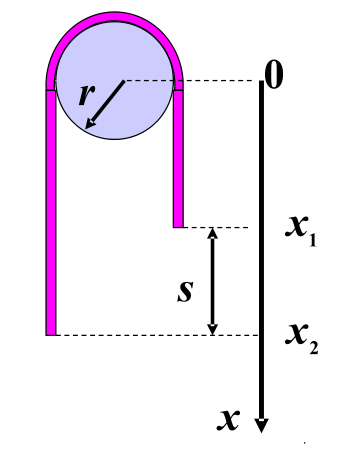
\includegraphics[width=0.15\textheight]{fig42}
        \caption{如图}\label{fig:42}
    \end{figure}
    \item 固定在一起的两个同轴均匀圆柱体可绕其光滑的水平对称轴$00^{'}$转动, 设大小圆柱的半径分别为$R$和$r$, 
    质量分别为$M$和$m$, 绕在两柱体上的细绳分别与物体$m_1$和物体$m_2$相连, $m_1$和$m_2$则挂在圆柱体的两侧, 如图所示\ref{fig:43}, 
    设$R=0.20m$, $r=0.10m$, $m=4kg$, $M=10kg$, $m_1=m_2=2kg$, 求柱体转动时的角加速度及两侧绳中的张力.
    \begin{figure}[h]
        \centering
        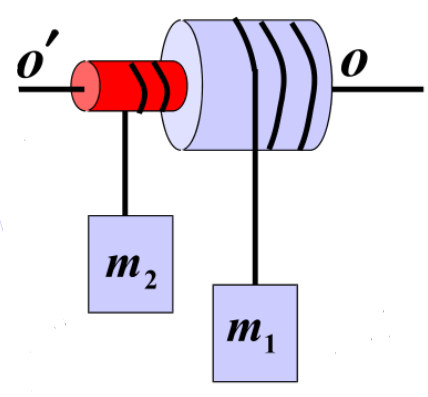
\includegraphics[width=0.15\textheight]{fig43}
        \caption{如图}\label{fig:43}
    \end{figure}
    \item 长为$L$的均匀细杆可绕过端点$O$的固定水平光滑轴转动.把杆抬平后无初速地释放, 杆摆至竖直位置时, 刚好和光滑水平桌面上的小球$m$相碰, 如图所示\ref{fig:44}, 
    球的质量和杆相同, 设碰撞是弹性的, 求碰后小球获得的速度.
    \begin{figure}[H]
        \centering
        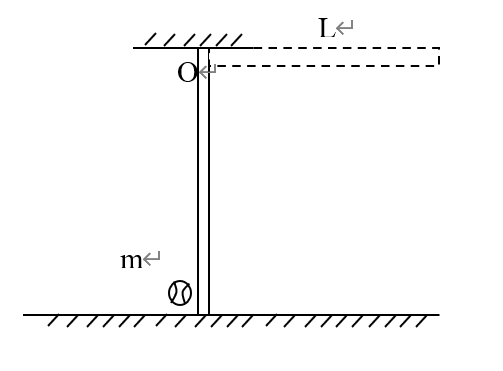
\includegraphics[width=0.15\textheight]{fig44}
        \caption{如图}\label{fig:44}
    \end{figure}
    \item 如图\ref{fig:45}, 一半径为$R=0.30m$, 质量为$M=15kg$, 质量均匀分布的圆柱体, 可绕与其几何轴重合的水平固定轴转动. 现以一不能伸长的轻绳绕于柱面, 而在绳的下端悬一质量
    $m=8.0 kg$的物体. 不计圆柱体与轴之间的摩擦, 求物体自静止下落$5s$内下降的距离.
    \begin{figure}[H]
        \centering
        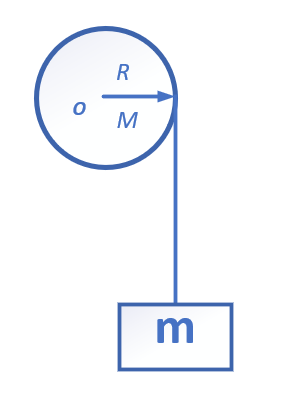
\includegraphics[width=0.15\textheight]{fig45}
        \caption{如图}\label{fig:45}
    \end{figure}
\end{enumerate}

\section{习题参考答案}
\subsection*{计算题}
\begin{enumerate}
    \item 质量为$M$的匀质圆盘, 可以绕通过盘中心垂直于盘的固定光滑轴转动, 
    绕过盘的边缘挂有质量为$m$, 长为$L$的匀质柔软绳索(如图\ref{Fig:42}), 
    设绳与圆盘无相对滑动, 试求当圆盘两侧绳长之差为$S$时, 
    绳的加速度的大小。
    \begin{figure}[h]
        \centering
        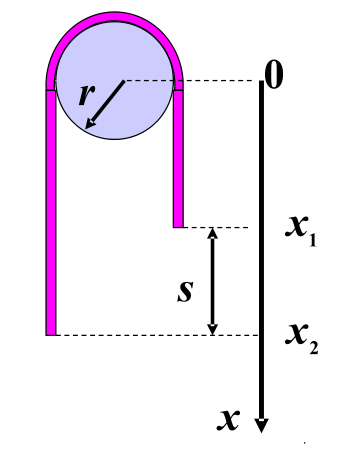
\includegraphics[width=0.15\textheight]{fig42}
        \caption{如图}\label{Fig:42}
    \end{figure}
    \begin{solution}
        看图: 
        \begin{figure}[H]
            \centering
            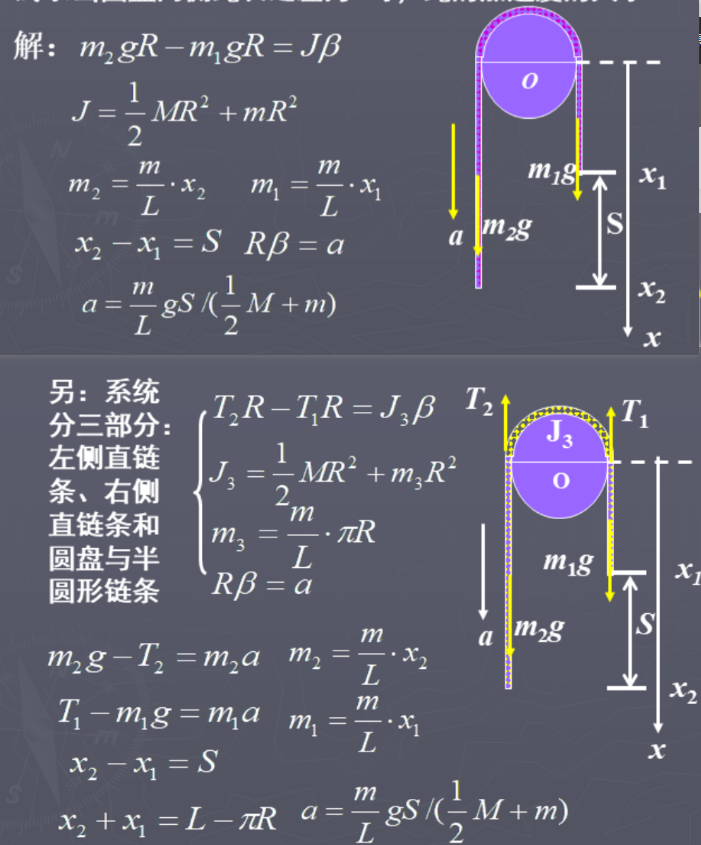
\includegraphics[width=0.48\textheight]{ans25}
        \end{figure}
    \end{solution}  
    \item 固定在一起的两个同轴均匀圆柱体可绕其光滑的水平对称轴$00^{'}$转动, 设大小圆柱的半径分别为$R$和$r$, 
    质量分别为$M$和$m$, 绕在两柱体上的细绳分别与物体$m_1$和物体$m_2$相连, $m_1$和$m_2$则挂在圆柱体的两侧, 如图所示\ref{Fig:43}, 
    设$R=0.20m$, $r=0.10m$, $m=4kg$, $M=10kg$, $m_1=m_2=2kg$, 求柱体转动时的角加速度及两侧绳中的张力.
    \begin{figure}[h]
        \centering
        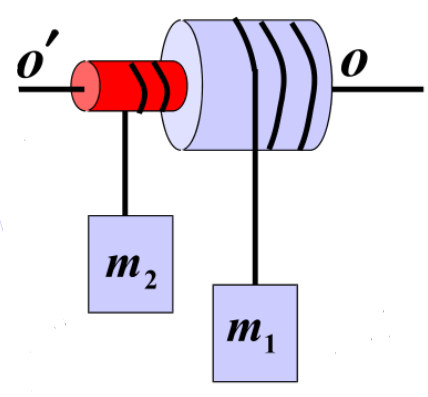
\includegraphics[width=0.15\textheight]{fig43}
        \caption{如图}\label{Fig:43}
    \end{figure}
    \begin{solution}
        看图: 
        \begin{figure}[H]
            \centering
            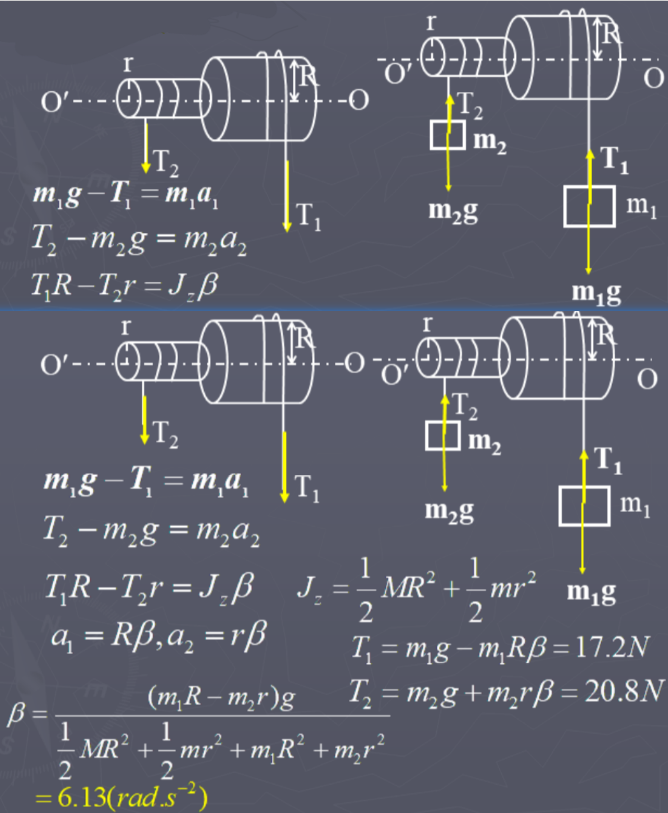
\includegraphics[width=0.48\textheight]{ans26}
        \end{figure}
    \end{solution}  
    \item 长为$L$的均匀细杆可绕过端点$O$的固定水平光滑轴转动.把杆抬平后无初速地释放, 杆摆至竖直位置时, 刚好和光滑水平桌面上的小球$m$相碰, 如图所示\ref{Fig:44}, 
    球的质量和杆相同, 设碰撞是弹性的, 求碰后小球获得的速度.
    \begin{figure}[H]
        \centering
        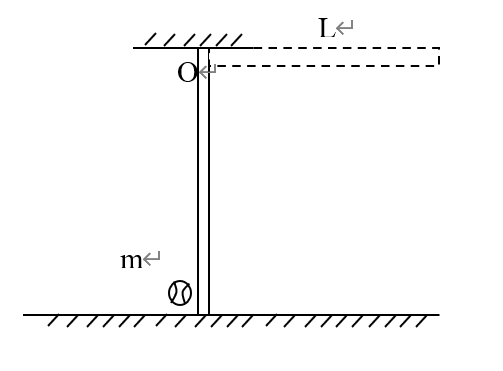
\includegraphics[width=0.15\textheight]{fig44}
        \caption{如图}\label{Fig:44}
    \end{figure}
    \begin{solution}
        看图: 
        \begin{figure}[H]
            \centering
            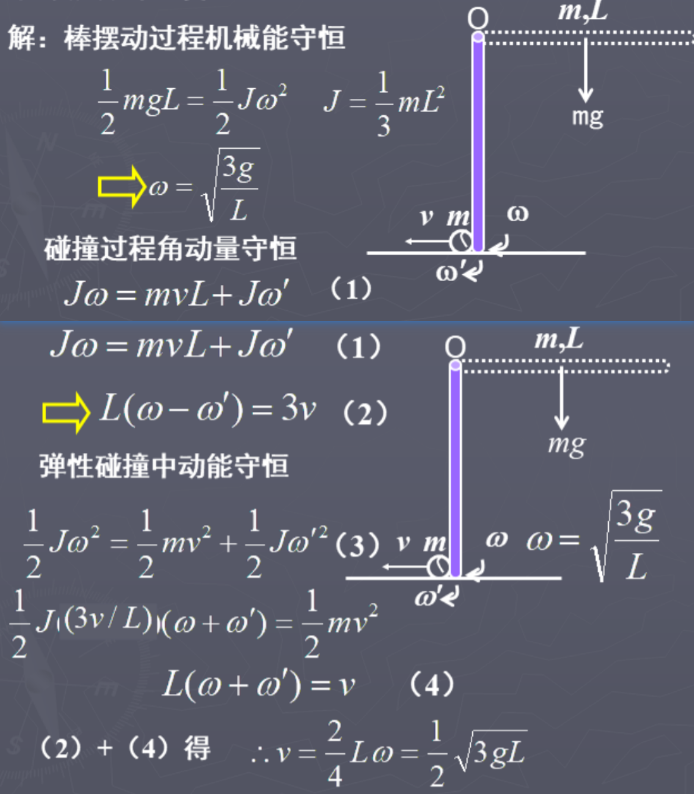
\includegraphics[width=0.48\textheight]{ans27}
        \end{figure}
    \end{solution}  
    \item 如图\ref{Fig:45}, 一半径为$R=0.30m$, 质量为$M=15kg$, 质量均匀分布的圆柱体, 可绕与其几何轴重合的水平固定轴转动. 现以一不能伸长的轻绳绕于柱面, 而在绳的下端悬一质量
    $m=8.0 kg$的物体. 不计圆柱体与轴之间的摩擦, 求物体自静止下落$5s$内下降的距离.
    \begin{figure}[H]
        \centering
        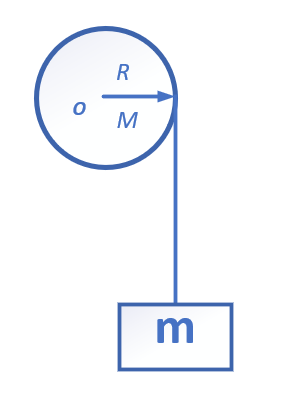
\includegraphics[width=0.15\textheight]{fig45}
        \caption{如图}\label{Fig:45}
    \end{figure}
    \begin{solution}
        看图: 
        \begin{figure}[H]
            \centering
            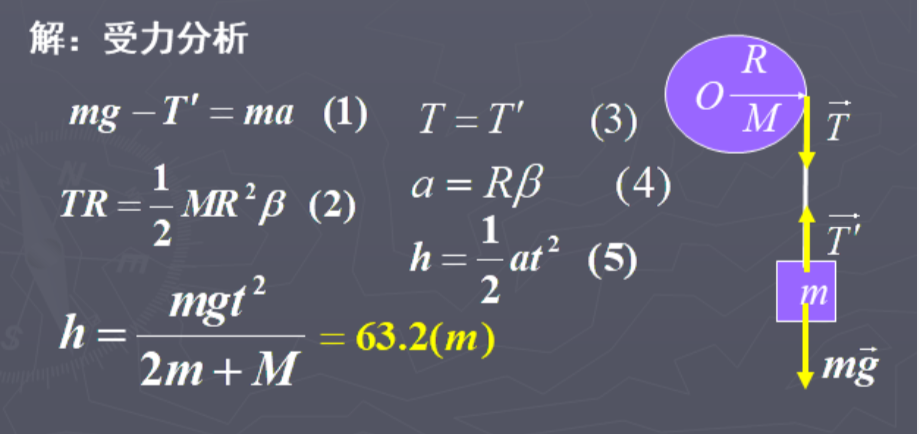
\includegraphics[width=0.48\textheight]{ans28}
        \end{figure}
    \end{solution}  
\end{enumerate}